\section{Decodable is not composable}\label{sec:phenomenon}
% CL1
\claim{CL1}
A one-step editor trained through the decoder (C1) decodes its target almost perfectly after one step (step-1 success at least
\CLoneVfiveCOneRoneMin{} in every BART cell of the fifth round), yet chains of two steps already fail: $\Rk{2}$ is at most
\CLoneVoneCOneRtwoMax{} over domains and seeds in the first round and \CLoneVfiveCOneRtwoMax{} on fresh worlds in the fifth (its sanity gate).
The closed-form RRR-16 operator, fitted only on canonical encoder pairs and never trained through the decoder, composes: its one-way
$\Rk{2N}$ is at least \CLoneVtwoRRRRtwoNMin{} on every domain of the second round and at least \CLoneVfiveBaseMin{} on every
(backbone, domain) of the fifth. One correct decoding step therefore says little about whether an edit can be repeated
(Figure~\ref{fig:fig1}).
\TODO{Table 1: main results summary across backbones and domains.}

\begin{figure}[t]\centering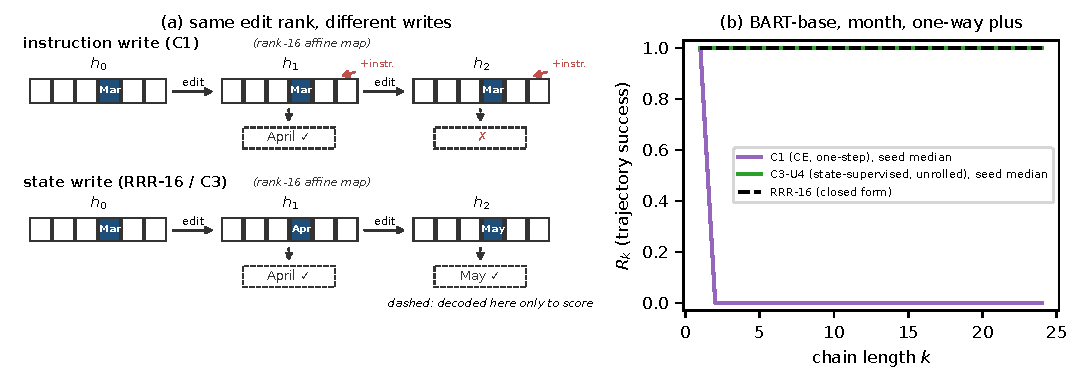
\includegraphics[width=\linewidth]{figs/fig1.pdf}
\caption{(b) BART-base, month, one-way plus chains: the one-step CE editor C1 fails from the second step; the closed-form RRR-16 and the
state-supervised unrolled C3-U4 compose. (a) \TODO{schematic}.}\label{fig:fig1}\end{figure}
